\chapter{POVQAD数据集构建}
\label{dataset}
本章旨在构建积木世界部分可见空间推理数据集,以便在后续研究中评估本文提出的神经符号VQA框架的性能,为本文的总研究目标服务。
下面分别就构建目标、构建准则、数据集定义、构建流程、数据集质量评估共五个方面展开介绍。
\section{构建目标}
本文提出构建一个积木世界部分可见场景空间推理数据集(Partial Observation VQA Data\-set, POVQAD)
,用于后续的研究中评估本文提出的神经符号VQA框架的性能。POVQAD的构建目标为:在部分可见积木世界场景下,通过遮挡、隐藏等设置,
考察模型结合背景知识和空间逻辑进行多步推理的能力。

以上数据集的构建目标,来源于以下几点:
\begin{enumerate}[nosep]
\item \textbf{CLEVR中场景信息完全可见}:对CLEVR中的某个问题而言,问题中涉及的所有物体,均在该问题对应的图像中
直接可见,不能反映现实世界中的部分场景可见的情形,不能满足本文研究目标中对于部分可见积木世界场景的需要。
例如,对于问题“What color is the cylinder to the left of the red sphere?”,
该问题对应的图像中左侧有一个蓝色圆柱体,右侧是红色球体。模型只需定位球体,并找其左侧物体,即可直接读取颜色。
\item \textbf{CLEVR缺少环境级逻辑约束}:CLEVR 场景中不存在“必须满足”的环境约束,
例如“所有红色物体必须是立方体”这类限制,使得推理任务缺乏积木世界空间推理中复杂性的模拟,不能考察模型综合利用背景知识进行系统推理的能力。
例如,对于问题“Are there more cubes than red things?”,
模型只需清点图像中立方体的数量和红色物体的数量即可比较并得出答案,而无需理解任何隐藏的逻辑条件或跨区域限制。
\item \textbf{CLEVR中问题的推理路径较短}:CLEVR中的很多问题只需一步推理或直接感知,不足以检验神经符号VQA框架在
积木世界多跳推理中的表现。例如,对于问题“What is the material of the small red object?”,模型只需要查找
图像中红色且尺寸为小的物体,即可直接回答材质,仅一次推理即可完成,推理路径很短。
\end{enumerate}
具体到数据集的各方面,构建目标可在图像、问题、环境约束、符号表示上进行进一步细化。
\subsection{图像层面目标}
图像层面上,具体包括以下目标:
\begin{enumerate}[nosep]
\item 设计部分遮挡和全遮挡两类图像。在实际VQA任务中,部分可见性是影响推理精度与鲁棒性的关键因素。
本文在构建POV\-QAD数据集时,特别关注两类具有代表性的“部分可见”情形——全遮挡图像和部分遮挡图像,并设计对应问题模板, 
以体现空间推理机制在不同可见性条件下的能力提升。

全遮挡图像属于“背景知识中已知,但图像中不可见”的情形。此类情形中,某些物体或其属性未出现在图像中,但依据环境布置的规则或先验知识,推理系统应当具备“补全”或“外推”能力。
例如:
\begin{enumerate}[nosep]
\item \textbf{背景约束}:场景中所有蓝色球体都放置在红色立方体后面,且每个红色立方体后面恰好有一个蓝球。
\item \textbf{图像内容(以文字描述)}:图中可见两个红色立方体,但它们后方区域被完全遮挡。
\item \textbf{问题示例}:这个场景中是否存在蓝色球体?
\end{enumerate}
尽管视觉输入中没有检测到任何蓝球,但根据背景规则和红立方体的数量,
系统应能得出“存在两个蓝球”的结论。这类问题强调的是利用背景知识进行结构性空间推理。

部分遮挡图像是“背景知识不足,且图像中被部分遮挡”的情形,这种情形代表了多数实际视觉任务中遇到的问题:
视觉系统可以检测部分被遮挡的物体,但缺乏对完整结构的观测,
难以仅靠视觉识别完成推理任务。本研究设计此类情境,旨在展示无需额外标注或监督,仅通过空间逻辑推理即可提升问答系统表现。例如:
\begin{enumerate}[nosep]
\item \textbf{图像内容(以文字描述)}:图中左侧有两个物体,其中一个绿色球体部分被另一个物体挡住,仅露出顶端。
\item \textbf{问题示例}:这个绿色球体是否位于红色立方体的上方?
\end{enumerate}
该情形下,仅凭部分视觉输入无法精确回答问题,但结合已有空间规则与遮挡顺序,系统可准确判断相对位置关系。
这类问题强调了空间逻辑推理在提升弱监督视觉问答中的作用。

因此,本文在POVQAD数据集中,特别设计了涵盖“背景知识可推理的完全不可见”和“无需标注即可推理的部分遮挡”两种部分可见情境,
以评估神经符号方法在复杂场景下的空间推理能力。
\item 保证高质量图像生成。本文设计的神经符号VQA框架中包含对图像的识别,需要根据识别出的物体以及物体之间的空间关系,
生成ASP规则以便后续针对不可见物体进行推理。因此能够准确、精准的识别可见的物体及其之间的关系,显得尤为重要,需要保证
图像以高质量水准生成,可见物体不能出现模糊、噪声等情况。
\item 将图像划分为多个区域。CLEVR没有对图像空间进行划分,不便于在空间层面定义一些约束条件,不能
充分考察模型的空间推理能力。通过将图像划分成若干个区域,可以将区域作为逻辑单元,便于定义局部或者跨区域的、全局的约束条件,验证
模型在空间层面上综合运用已有条件,进行逻辑推理的能力。
\end{enumerate}
\subsection{问题层面目标}
问题层面,具体包括以下目标:
\begin{enumerate}[nosep]
\item 以信息缺失物体为核心设计问题。CLEVR中的问题大多围绕图像中的完全可见的物体,即
回答该物体相关的问题的所需信息,全部都包括在图像中。CLEVR中的这一问题,导致CLEVR中缺少信息缺失的情境下的推理。
围绕信息缺失物体设计问题,可以引导模型进行推理、归纳,而非直接对图像进行感知并回答问题,考察模型的逻辑推理能力。
\item 控制问题类型分布。CLEVR中,物体的某些属性的问题的可能答案太少,例如关于材质的问题的可能答案仅有两种,
而颜色与形状的属性可取值较多,对应其相关问题的答案集空间更大,模型通过随机猜测命中的正确答案的概率大大降低。
故要对问题类型进行合理控制,尽可能扩大答案集空间,提高模型在“多值不确定性”下的能力。
\item 覆盖多种推理类型。CLEVR中的很多问题只需一步推理或直接感知,不足以检验神经符号VQA框架在
积木世界多跳推理中的表现。通过在POVQAD中设计不同推理跳数的问题,可以测试模型对链式逻辑的掌握程度。
\item 不直接通过“A在B的哪个方向?”这一类直接提问空间关系的问题,而是间接地设计问题来考察模型的空间推理能力。这一做法有以下几点原因:

(1)模拟真实场景中的不完全信息推理需求。在现实世界中,空间关系的应用经常是隐性的,不是直接问“哪个在左边”,而是:
“这个红球下面是什么?”或“最右边的立方体是什么颜色?”
但当部分场景不可见时,要想回答这类问题,模型就必须结合场景中已有的部分信息和环境约束进行空间补全和逻辑推理,
这实际上就考验了模型是否掌握了空间关系。而本文的问题中,目标物体(即被提问的物体)和参照物体(图像中信息完全,用来作为参照物的物体)
之间的关系均通过空间关系(上、下、左、右或者所在物体区域)来建立。如果要回答POVQAD中的问题,就必须要运用空间关系。

(2)防止模型直接记忆答案模式。如果问题中直接写明“左边的物体是什么”,模型可能只靠表面的模式学习就能答题,而不需要空间推理能力。
通过在问题设计上设置空间关系而不是直接提问,可以迫使模型“用上空间推理”而不是“看图找答案”。

(3)展现符号方法在空间推理方面的相对优势。本论文的研究目标之一是促进神经符号方法的发展。
直接提问空间关系可能会让纯神经模型也能勉强处理,而通过间接考察的方式,更有利于展现符号方法(如ASP)在空间建模方面的优势,
尤其是在显式表示空间约束、进行场景补全推理、得出结论的可解释性方面。
\end{enumerate}
\subsection{约束层面目标}
约束是对场景中对象空间配置的规则限制,定义对象之间的空间关系或位置要求。
每条约束基于一个约束模板实例化得到,具有明确的逻辑语义。
约束层面,具体包括以下目标:
\begin{enumerate}[nosep]
\item 使用ASP构建背景知识约束。CLEVR中对某个图像而言,缺少对其相关背景知识的设定,
进而无法考察模型是否能真正整合场景逻辑进行思考。而构建规则正是ASP的长处所在。
\item 模版化建模,支持约束组合多样性,形成多样化的环境。
CLEVR中。一方面对图像内物体数量、物体属性取值空间等要素均进行了参数化处理,可以自定义修改,另一方面支持多个模板之间的自由组合。
两种方法搭配,增加了环境的多样性。
\end{enumerate}
\subsection{符号表示层面目标}
符号表示层面的目标为:使用ASP进行统一编码。ASP是神经符号VQA框架的核心所在,在框架内部全程使用ASP进行知识表示,
能够有效减少不同知识表示形式之间进行转换而带来的损耗,保证知识的完整性。
\section{构建准则}
本文旨在构建一个部分可见积木世界场景的空间推理VQA数据集(POVQAD),用以模拟
现实世界中信息缺失的场景,并评估模型的空间推理能力。为实现该目标,本文在POVQAD数据集的构建中
遵循如下准则:
\begin{enumerate}[nosep]
\item 每个场景中有一个目标物体被隐藏,图像和逻辑表示中均不可见。场景指的是图像的ASP表示,其中包含了图像的物体属性及各物体之间的空间位置关系。
隐藏物体的目的是为了实现部分可见性,模拟现实中因遮挡或感知局限导致的信息缺失情境。
\item 每个场景都必须满足由 ASP 定义的一组环境约束,目的是保证场景内部在逻辑层面上的合理性,避免不同约束之间发生冲突。
例如,不能同时出现“区域1中所有物体都是蓝色”和“区域1中没有蓝色的物体”这种自相矛盾的约束。
\item 在环境约束定义、场景生成与问题的形式化表示方面,均采用ASP进行表示。原因在于以下几方面:

ASP支持高层次知识建模。POVQAD所涉及的空间推理任务,本质上是一个多层次的知识表示与约束求解问题。
环境约束定义了某类场景中物体属性分布的全局或局部规则;场景构建要求从这些规则中生成满足逻辑一致性的物体布局;
问题表示与求解则需要基于观察到的部分信息,反推出隐藏物体的属性。
在这些任务中,ASP具有以下核心优势:(1)声明式建模,使用逻辑规则直接描述“应该满足什么”,
而不是“如何计算”,避免编程过程的冗余细节;(2)非单一模型求解,ASP可自动求解所有满足条件的模型,天然适合多解推理任务;
(3)支持不完备信息建模,通过否定与缺省推理机制,可以有效表示部分可见性下的场景;
(4)可组合性强,环境约束、已知信息与问题查询均可通过逻辑程序合并输入,实现统一推理。

在环境约束生成中,ASP能够高效表达复杂的属性限制。环境约束可能包括限制属性取值(如“区域0中所有物体必须是红色或黄色”)、
限制物体数量(如“区域1中恰好有2个小物体”)、跨区域比较(如“区域1和区域2中相同颜色的物体数不能超过3”)以及
排他性限制(如“不得存在两个属性完全一致的物体”)。这些约束结构灵活,复杂度高,传统的数据生成方法难以精确表达。而 ASP 的规则语法(例如 :- 引入约束,\#进行计数等)非常适合表达此类逻辑条件。

在场景构建中,ASP可有效保障逻辑一致性。在场景构建过程中,ASP求解器被用作生成器,即在给定环境约束的前提下,
通过ASP求解器获得符合约束的场景。每个完整场景对应一组ASP事实;ASP求解器在物体属性组合与区域位置上
进行求解;最终仅保留满足所有约束条件的合法解集,用于渲染与问题生成。通过在场景构建中使用ASP求解器,
可以系统性地采样出大规模、逻辑一致、属性多样的积木世界场景,避免人工构造或启发式方法中可能出现的歧义与逻辑错误。

在问题表示中,ASP实现了可求解性与可解释性的统一。POVQAD中的问题不仅以自然语言形式存在,
还被转换为对应的ASP查询规则,这一方案的优势包括:(1)问题可直接嵌入ASP推理流程,与部分场景信息与环境约束统一求解;
(2)保证所有问题均具有可求解性:Clingo 求解器可验证其是否有合法答案;(3)通过分析解集大小、排除路径等,可进行问题难度分级与推理链可视化;
(4)每个问题的“答案空间”明确,适用于多解式评估与开放性回答。例如,问题“What is the color of the object with the same material as the object to the right of the red sphere?”可形式化为:
\begin{lstlisting}
query(Q) :-
  has_property(X, color, Q),has_property(X, shape, cylinder),
  has_property(Y, shape, sphere),has_property(Y, color, red),
  right(Y, X),same_material(X, Y),X != Y.
\end{lstlisting}
这种形式使得问题的语义清晰、结构明确,便于执行与验证。
\item 图像中物体属性设置形状、尺寸、材质、颜色四种属性。具体属性值的设置上,尺寸的可能取值为小、中、大,颜色的可能取值为红色、蓝
色、绿色、黄色、灰色、棕色、紫色和青色,材质的可能取值为橡胶和金属,形状的可能取值为圆锥体、球体、圆柱体和立方体。

选取这四种基本属性,是因为它们是物体最直观且容易区分的特征,并且与原始 CLEVR 数据集保持一致,便于进行比较研究。对
每个属性的可能取值进行了限制(例如,八种颜色,四种形状,两种材质,三种尺寸),
这样做的目的是为了简化推理过程并控制答案的搜索空间,避免由于可能的属性组合过多而导致的推理复杂度过高。
\item 图像中对空间进行划分,并分为四个区域,取值分别为0、1、2、3,并同时规定每个物体只能在图像的一个区域中,不能同时跨多个区域。
为图像空间划分区域,主要的优势在于为图像生成和问题生成指定作用范围约束,有利于提升数据集的复杂性和多样性。
\item 问题类型删除了CLEVR中的是否类问题(即比较属性、比较数量和存在性问题)以及计数问题,仅保留属性查询类问题。
做出这一规定的原因在于以下三点:

(1)POVQAD 的核心目标是评估模型在部分可见积木世界场景中进行空间推理的能力。
相比布尔值或数字作为结果的“是否类”与计数问题,
属性查询问题更能体现模型如何结合部分观测信息与环境约束,排除不符合条件的选项,最终推理出不可见物体的属性。

(2)是否类问题和计数问题的答案通常是“是/否”或整数,ASP 系统在求解这类问题时所涉及的推理路径较为简单
,缺乏中间可解释的逻辑链,难以体现复杂的空间推理过程。
而属性查询问题往往需要经过一系列基于已知信息的假设、排除、归纳等推理步骤,可以更完整地展现 ASP 系统的推理能力和可解释性。

(3)从实际教学与评估角度出发,属性查询问题有助于更好地分析模型失败的原因,
便于定位是视觉理解错误、知识调用缺失,还是逻辑链条断裂;而布尔类问题的回答更难反推推理过程中的缺陷。

因此,为更精准地衡量模型在复杂空间推理任务中的表现,并提升神经符号方法的可解释性与诊断性,本文在 POVQAD 中仅保留属性查询类问题。
\end{enumerate}
\section{数据集定义}
基于上述构建目标,本文将POVQAD数据集形式化定义为一个五元组的集合:
$$D = \{ (I_i,P_i,Q_i,\Pi_i ,A_i) | i=1,2,...,N \}$$
其中,每个元素$(I_i,P_i,Q_i,\Pi_i ,A_i)$是数据集中的一个样例,各组成部分定义如下:
\begin{enumerate}[nosep]
\item \textbf{$I_i$}为图像,是通过 Blender 渲染的基于场景生成的 3D 图像。
每张图像表示一个三维积木世界场景,所有可见物体均按预定义属性摆放。每个图像中都刻意隐藏了一个物体,以模拟部分可见条件。
图像示例如图\ref{POVQAD-figure}。
\begin{figure}
\centering
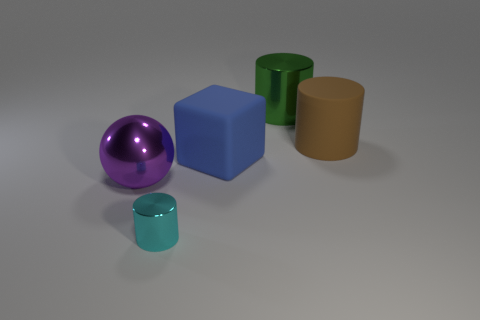
\includegraphics[scale=0.6]{figures/POVQAD中图像示例.png}
\caption{POVQAD中图像示例}
\label{POVQAD-figure}
\end{figure}
\item \textbf{$S_i$}为场景,是对当前图像中所有可见物体的ASP表示,采用ASP进行表示。
其中主要包含以下内容:每个可见物体的属性,包括尺寸、颜色、材质、形状;每个物体所属的区域;可见物体之间的空间关系,如\textbf{left(X,Y)}表示X在Y的左边;
被隐藏的物体(即问题中提及而图像中不存在的物体)不会出现在部分场景信息中。
\item \textbf{$Q_i$}为问题,使用自然语言形式进行表示,例如“What shape is the small red object that is to the left of the yellow cube?”。
所有问题均为属性查询类问题,专门针对物体的四个属性之一:颜色、尺寸、形状或材质。
\item \textbf{$QA_i$}为问题的ASP表示,例如:
\begin{lstlisting}
query(Q) :-
  has_property(X, color, Q),has_property(X, shape, cylinder),
  has_property(Y, shape, sphere),has_property(Y, color, red),
  left(Y, X),same_material(X, Y),X != Y.
\end{lstlisting}
\item \textbf{$\Pi_i$}为环境,是当前图像所属环境的一组约束规则,采用ASP进行表示。以下为一组约束示例:
\begin{lstlisting}
% 约束示例
% 区域0中所有物体的形状必须是圆柱体
:- obj(X), at(X, 0), has_property(X, shape, cylinder).
% 区域1中蓝色物体的数量大于2个
:- #count{X: has_property(X, color, blue), at(X, 1)} > 2.
\end{lstlisting}
\item \textbf{$A_i$}为答案集,表示该问题对应的正确答案。
\end{enumerate}
\section{构建流程}
POVQAD的构建流程如图\ref{fig:dataset-generation}所示,共包括5个步骤。各个步骤的功能如下:
\begin{enumerate}[nosep]
\item \textbf{生成环境}:随机选取部分约束模板,并将模板实例化,最终得到环境。
\item \textbf{构建场景图}:将环境实例化,并将环境输入ASP求解器进行求解,分别生成部分可见场景图和不可见场景图。
\item \textbf{图像渲染}:使用Blender对场景图进行渲染,获得积木世界图像与场景。
\item \textbf{问题生成}:根据问题模板与场景生成问题与其对应ASP查询,并使用Clingo得到问题的解,此外对答案集进行筛选。
\end{enumerate}
\begin{figure}[h]
\centering
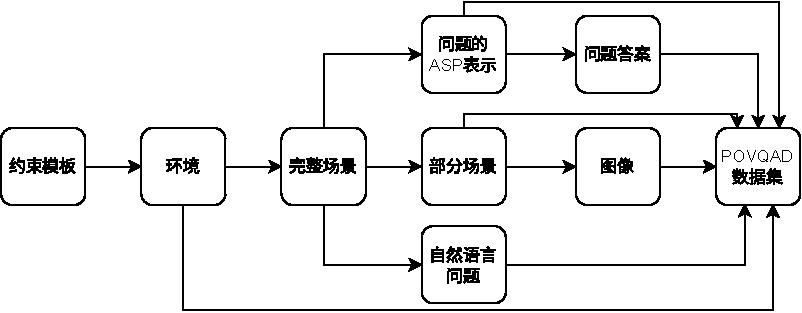
\includegraphics{figures/pipeline-POVQAD.drawio-crop.pdf}
\caption{POVQAD构建流程}
\label{fig:dataset-generation}
\end{figure}

\subsection{生成环境}
在POVQAD中,一个环境包含了一组约束规则,用于限定在该环境下生成的所有场景所必须满足的
属性组合、区域位置的约束条件。环境的作用是,在宏观层面上对后续生成的图像、问题进行把控,
以控制场景复杂度,并保证数据集保持逻辑一致性。在数学上可以如下表示环境:
$$ \varepsilon = \{C_1,C_2, ..., C_k \}, C_i \in ASP \quad Constraint $$
其中,每个$C_i$是用 ASP 表示的一条逻辑约束规则。

环境的生成过程包括以下步骤:(1)预定义11种约束模板;(2)确定模板中的相关参数;(3)对所有生成的约束经语义检查与逻辑一致性验证。

约束模板是依据常见的逻辑组合来进行设计的,覆盖了取值限定、逻辑否、逻辑或等基本逻辑模式,
部分约束模板的ASP编码表示以及对应表示含义见表\ref{tab:asp_templates},全部约束模板见附录\ref{appendix:constraints}。
除了约束模板之外,还有全局约束。
全局约束是所有生成的环境都应遵循的约束,对整个积木世界进行了基本定义,例如“平面区域划分为4个,编号0、1、2、3。”就是通过全局约束定义的,
ASP形式为\texttt{region(0). region(1). region(2). region(3).}。
本文所用的所有全局约束在附录\ref{appendix:environment}同样予以了展示。
\begin{table}[h]
    \centering
    \renewcommand{\arraystretch}{1.0}
    \begin{tabular}{|p{2.8cm}|p{12.2cm}|}
        \hline
        \textbf{模板} & \textbf{描述} \\
        \hline
        \textbf{模板1(取值约束)} & 
        \texttt{:- obj(X), at(X, R), not has\_property(X, P1, V1).} \\ 
        & 解释: 对区域R中的所有物体,它们P1属性的取值均为V1。 \\ 
        & 具体实现: :- obj(X), at(X, 0), not has\_property(X, color, red). \\
        \hline
        \textbf{模板2(遮挡比例约束)} & 
        \texttt{:- occlusion\_rate(T, R), (R <= 0; R >= 1).} \\ 
        & 解释:物体T被遮挡的比例为R(0<R<=1),完全遮挡时R=1。 \\ 
        & 具体实现::- occlusion\_rate(T, 0.1). \\
        \hline
    \end{tabular}
    \caption{部分约束模板示例}
    \label{tab:asp_templates}
\end{table}

模板实例化生成环境的过程中,需要设定一些参数,具体包括:
\begin{enumerate}[nosep]
\item \textbf{规则模板数量}:每个环境实例化多少条规则模板,规定单个环境最多实例化15条。
\item \textbf{属性类型}:将模板中的属性类型占位符用实际生成的属性类型进行替换,例如 P1' 替换为 color,P2' 替换为 shape。
\item \textbf{属性值}:用随机生成的属性值替换,例如 V1' 替换为 red,V2' 替换为 sphere。
\item \textbf{区域范围}:规则作用在哪些区域。根据POVQAD的定义,区域编号为0、1、2、3。
如果是全局作用的模板,则需要将该条规则的作用区域设置为0、1、2、3。如果是作用在局部区域,仅需设置某个或某几个区域即可。
\item \textbf{数量参数}:恰有、至少、至多约束中要求的具体数量。
\end{enumerate}

模板实例化之后,再基于所得的模板实例,为每个区域生成区域内约束,并随机生成跨区域约束和强制否定约束。
强制否定约束用于限制某些属性或者属性做个不能出现在特定区域中,跨区域约束用于限制多个区域之间对象的关系或者属性分布,区域内约束
用于限制单个区域内对象的属性或者属性组合。
最终,得到具体的约束表达式如下所示:
\begin{lstlisting}
:- object(X), at(X, 0), not hasProperty(X, color, red).
:- object(X), at(X, 1), hasProperty(X, shape, cube).
:- #count{sameProperty(X1, X2, color): object(X1), object(X2), at(X1, 0), at(X2, 1)} < 2.
\end{lstlisting}

POVQAD规定每个环境最多由15条约束规则模板实例化构成,这一数值是经过多方面权衡确定的,目的主要在于以下几方面:
\begin{enumerate}[nosep]
\item 逻辑复杂度与可解性的平衡。如果某个环境中的约束规则过少,会导致后续生成的场景过于松散,
物体属性组合高度自由,推理空间过大,导致问题复杂度过大,难以进行有效推理。
如果约束规则过多,则会造成约束之间产生冲突,导致ASP求解器难以知道合法的解,影响求解效率,进而影响场景的生成。
\item 控制生成时间与可维护性。每条规则在 ASP 中都可能极大影响解空间,规则数上升将显著增加 ASP 求解时间。此外,
在大规模数据生成中,15 条以内的环境可以在数秒内稳定求解出场景,利于批量生成和调试。
\end{enumerate}

在生成环境的过程中,规定每个环境中至少包括区域级约束和跨区域约束,共计两种约束。做出这一规定的目的在于
增强环境的逻辑层次性与推理深度,具体原因如下:
\begin{enumerate}[nosep]
\item 支持多层次推理链的构造。区域级约束用于构建局部一致性,跨区域约束用于建模全局对比或协同关系。
同时使用这两类约束,可以使推理问题具有从局部到跨区域的空间层级,增加问题的空间深度。
\item 避免场景构造退化为简单的组合。如果只使用区域级约束,那么后续根据环境生成场景时,将会变成多个局部区域的简单组合,
缺乏各个区域之间的相互关联。添加跨区域约束之后,有助于生成具有全局一致性/相互限制/相互支撑的复杂场景。
\item 支撑部分可见场景下的间接推理。在部分场景中,若不可见物体在区域0中缺失,模型可以通过区域0的其它规则
或者区域0与区域1的对比或者联动规则来进行属性排除或依存判断。而如果采用单一的区域级约束,
那么对于区域0中的物体的问题,模型只能依赖于区域0的局部信息进行推理,缺乏全局视角,不利于考察模型的宏观层面推理能力。
\end{enumerate}

此后在生成环境时,将全局约束与获得的约束表达式进行拼接,形成完整ASP程序,并由Clingo对ASP程序进行求解。
如果Clingo的输出至少存在一个答案集,说明当前约束可满足,将所得结果(即环境)保存到ASP程序的\texttt{.lp}文件中。如果Clingo没有答案集,说明当前约束不满足,会
尝试使用其它的约束表达式进行求解,直到能够生成一个环境。

进行语义检查与逻辑一致性验证的具体方案是用ASP求解器(本文中采用Clingo)对生成的约束尝试进行求解,
如果Clingo没有提示错误信息,并且能够成功求解出至少一个合法的解集,则说明该环境的约束规则是逻辑一致的,并且
能够顺利通过语法检查。本步骤的主要目标是避免后续出现死循环、空解等问题。

最终,一共生成了30个环境,数据集中的所有场景均匀分布在这些不同的环境之中。
控制生成30个环境的原因是,这一数量的环境实际上可以供后续生成数百万个不同场景和问题,足够支撑进行大规模训练与严格测试。
环境的具体示例见附录\ref{appendix:environment}。
\subsection{构建场景}
\subsubsection{构建完整场景图}
在获得环境约束后,需要进一步获得符合约束的场景图,所需流程为:
将获得的环境约束Clingo进行求解,生成符合约束的答案集,并对答案集进行采样。一个答案集
对应一个完整场景图。此后,将答案集进行解析,获得完整场景图。

首先,将包含了环境约束的\texttt{.lp}文件提交至Clingo进行求解,对Clingo的输出结果进行简单解析,将所有答案集进行提取。

在生成答案集之后进行采样出于以下两点原因:
\begin{enumerate}[nosep]
\item 避免处理过多的答案集。如果直接处理所有答案集,会导致后续的场景生成和问题生成过程耗费大量时间和资源。
\item 控制场景的多样性。如果直接使用所有答案集,可能会生成大量相似的场景,导致数据集的多样性不足。
某些约束可能会导致生成的场景具有高度重复的物体属性或关系。随机采样可以增加场景的多样性,避免生成过于相似的场景。
\item 平衡约束类型的答案集。不同的约束类型可能会生成不同数量的答案集。
如果某些约束类型生成的答案集过多,而其他约束类型生成的答案集较少,可能会导致数据集中某些类型的场景占比过高。
对每种约束类型的答案集进行采样,可以平衡不同约束类型的场景数量,确保数据集的均衡性。
\item 降低后续处理的复杂度。每个答案集需要进一步解析为场景图,并用于生成图像和问题。
如果答案集数量过多,会显著增加后续处理的复杂度。通过减少答案集数量,降低后续处理的复杂度,确保生成管道的可控性。
\end{enumerate}

场景是最终渲染的图像及其对应的描述信息,包括图像中的所有物体及其属性和位置。场景以JSON文件存储,某个场景如下所示:
\begin{lstlisting}

\end{lstlisting}

场景图是场景的结构化表示,描述了场景中物体的属性以及物体之间的关系,是场景的一种中间表示。某个场景图如下所示:
\begin{lstlisting}
{
  0: {"color": "red", "shape": "sphere", "size": "large", "material": "rubber", "region": 0},
  1: {"color": "blue", "shape": "cube", "size": "small", "material": "metal", "region": 1}
}
\end{lstlisting}

对答案集进行解析的过程实际上是对谓词进行解析的过程,会将\texttt{has\_property}和\texttt{at}两个谓词进行解析,
最终形成以JSON格式存储的场景图。

此后基于所得的完整场景可以生成部分可见场景和不可见场景。以下两小节将展开介绍。
\subsubsection{构建部分可见场景图}
部分可见场景与完整场景的区别在于:部分可见场景中增加了对于物体之间遮挡关系以及遮挡比例的规则,进而后续Blender根据场景
渲染图像时,能够得到场景中描述的部分物体之间存在遮挡的图像。构建部分可见场景的具体流程如下:

首先从完整场景中,随机选取两个物体,并分别指定一个物体为将会被提问的目标物体\texttt{T}
,另一个物体为去遮挡目标物体的\texttt{Oc}。
此后,向场景中添加ASP谓词\texttt{target(T)}、\texttt{occluder(Oc)}以及\texttt{occludes(Oc,T)},分别表示
\texttt{T}为目标物体,\texttt{Oc}为遮挡物体,Oc在图像中遮挡了T。此后,生成一个介于0和1之间的随机数$R$,用于表示目标物体
被遮挡的面积比例。本文规定$R$大于0且小于1。当$R=1$时,相当于目标物体被完全遮挡,对应不可见场景的构建,为其它不同的构造方法。

此后,再随机选择目标物体\texttt{T}的形状、颜色、材质、尺寸中的任意一个属性,将其从场景中移除,以表示由于该物体被遮挡导致的信息缺失。
\subsubsection{构建不可见场景图}
基于完整场景构图建不可见场景图的构造思路是:从完整场景图中随机移除一个对象。

本环节的目标是,从完整场景中随机选择一个物体作为被隐藏的目标物体,并围绕该物体构造相关问题
,并同时使用自然语言及ASP对问题进行表示。
整个环节的流程图如\ref{generate-partial-scenes-and-questions}所示。
\begin{figure}[h]
\centering
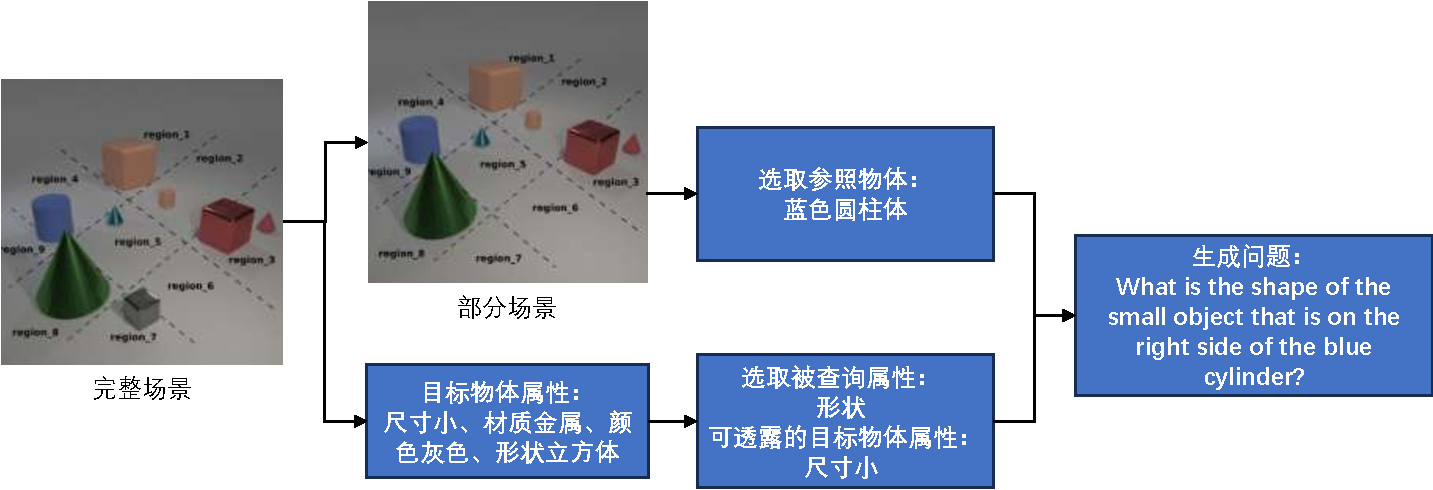
\includegraphics[scale=0.6]{figures/部分场景及问题生成-crop.pdf}
\caption{构建部分场景并生成问题流程图}
\label{generate-partial-scenes-and-questions}
\end{figure}

选择目标物体的过程需要满足以下条件:
\begin{enumerate}[nosep]
\item 从完整场景的所有物体中随机选取一个,在随机选取的过程中,要注意保持均衡,不能
一直选取单一区域的物体或者相同属性的物体,以免造成数据偏态分布。
\item 被选择物体不能是唯一出现某一属性的对象,避免由于移除该物体后,
导致场景中该属性的值无法被推断,导致问题无解。
\item 该物体将在后续问题中作为查询目标。
\end{enumerate}

选择$Obj_i$后,需要将完整场景中关于$Obj_i$的所有事实全部移除,生成部分场景。具体需要做到以下几点:
\begin{enumerate}[nosep]
\item 删除\texttt{obj(i)}、\texttt{at(i, R)}、\texttt{has\_property(i, P, V)};
\item 删除所有涉及$Obj_i$的空间关系谓词,如\texttt{left(i, j)}、\texttt{right(i, j)}等;
\item 保留其余物体的信息与关系。
\end{enumerate}
从而得到一个只包含可见物体的子结构,记为 $Partial_i$,该场景中缺少了目标物体的显式信息。

随后,将根据$Obj_i$的属性来生成相关问题。
每一个生成的问题,应该满足如下条件:(1)针对被隐藏对象的某一属性;
(2)基于剩余可见物体和环境约束进行间接推理;(3)问题语义必须明确且答案集非空。
以某个问题的生成为例,$Obj_i$的属性包括:尺寸为小、材质为金属、颜色为灰色、形状为立方体
,那么可以随机选取形状作为被查询属性,并将“尺寸为小”作为已知信息放置在问题当中。
为了便于控制问题类型的数量分布,本文规定每个问题只能查询上述四个属性中的一个,而不同时查询多个属性。
与此同时,问题生成器也将从图中选取一个
参照物体,用以共同组成问题。考虑到不同种类属性的可能取值数量不同,进而不同属性的问题的可能答案数量也不同,
本文据此规定每种属性的问题在数据集中所占的比例:颜色与形状各占40\%,材质与尺寸各占10\%。
该比例同样通过ASP约束来进行实现。
需要注意生成的问题仅为属性查询问题,不包括是非题和计数题等其它CLEVR中原有的问题类型,理由在3.1节构建目标中已有陈述,此处不再赘述。

\subsection{图像渲染}
图像渲染与样例生成的目的是将部分可见场景图以及不可见场景图转换为场景,并使用Blender进行渲染。

\begin{enumerate}[nosep]
\item 初始化Blender渲染对象。在这一步中,主要是设置一系列渲染参数,包括分辨率、GPU设置等等。
\item 定义场景字典。该字典中保存了场景的元信息(即将生成的图片名称等)、物体信息和方向信息。
\item 方向向量计算。先获取在场景初始化时添加的平面的法向量,此后计算摄像机的方向向量,并将
摄像机的方向向量投影到平面上,得到相对于平面的方向向量。计算完成之后,将平面删除,避免影响后续渲染
\item 向场景中添加物体。根据场景图中的物体信息,将物体添加到场景中。添加过程中,要注意确保物体之间的距离和边距满足约束条件。
此外,在生成部分可见场景时,要注意根据部分可见场景图中的遮挡物体和遮挡面积比例,来生成遮挡的情形;
在生成不可见场景时,要注意。
\item 计算物体之间关系。基于物体的三维坐标和场景的方向向量,遍历场景中的每对物体,
计算得出空间中上、下、左、右、前、后等关系。判断两个物体之间是否存在某种关系的阈值设置为0.2,即如果两个物体之间的
方向向量的点积大于0.2,那么认为它们具有该关系。

最终,输出一个JSON对象,其中描述了场景中所有物体之间的空间关系,一个可能的字典如图所示,其中$left[0] = 1$说明
物体0的左侧有物体1,$right[1] = 0$说明物体1的右侧有物体0。
\begin{lstlisting}
{
    "left": [[1], [], [], []],
    "right": [[], [0], [], []],
    "above": [[], [], [3], []],
    "below": [[], [], [], [2]],
    "front": [[], [], [], []],
    "behind": [[], [], [], []]
}
\end{lstlisting}
\end{enumerate}

在图像渲染完成之后,整个场景构造完成,此时进行数据整合,将所有场景文件合并同一个包含所有场景的JSON文件中。

\subsection{问题生成}
POVQAD根据前述步骤整合的场景文件和问题模板来构造自然语言问题,
一种供参考的模板如\ref{asp:question-template}中所示,
其中<Z2>、<C2>、<M2> 表示待查询对象的已知属性(例如尺寸、颜色、材质),由随机策略从完整场景中选取;
<R> 为空间关系(如left、right、front、behind),其取值既满足随机性,又依赖于完整场景中物体间的真实空间分布;
<Z>、<C>、<M>、<S> 则代表参考对象的属性。这种模板化设计不仅使自然语言问题的结构化描述成为可能,
而且便于后续转换为ASP的形式化表示,从而实现问题求解的自动化。
\begin{lstlisting}[label=asp:question-template]
What shape is the < Z2 > (size) < C2 > (color) < M2 > (material) [that is] 
< R > (relation) the < Z > (size) < C > (color) < M > (material) < S > (shape) ?
\end{lstlisting}

首先,筛选问题模板。对模板的筛选,按照模板的查询目标是否与当前场景相匹配,以及模板中给定信息是否在场景中存在来进行。例如,对于下列问题模板,其提问的是
“物体A是否在物体B的上方?”但是该场景图中,两物体之间的
\begin{lstlisting}

\end{lstlisting}

问题模板筛选完毕之后,根据场景图和筛选好的问题模板,进行模板实例化,生成问题文本及其对应的ASP查询。
实例化过程中,需要对模板中的占位符替换为具体的属性值。对每一个自然语言问题,都是从一个问题模板出发,填充占位符,
然后生成的。所以,自然语言和ASP查询具有一一对应的逻辑结构,可以实现自动转换。

此后调用Clingo求解查询,生成问题的答案,并通过对答案进行分析,实现对生成问题的筛选。
筛选逻辑是:如果答案集为空或者包含所有的可能值,则丢弃当前问题。对生成问题进行筛选有以下三点原因:
\begin{enumerate}[nosep]
\item 提高问题的质量。确保生成的问题有明确的答案,而不是模糊或无意义的问题。
\item 避免冗余问题。避免生成答案集过大的问题,这些问题可能对模型训练没有帮助。
\item 确保问题的多样性。筛选掉覆盖所有可能答案的情况,确保问题具有一定的区分性。
\end{enumerate}

最后,将生成的问题、ASP查询和答案保存为JSON文件,以下为一个示例:
\begin{lstlisting}
{
    'split': scene_info['split'],
    'image_filename': scene_fn,
    'image_index': image_index,
    'question': ts,
    'program': qs,
    'asp_query': asp_query,
    'answer': possible_sols,
    'object_interest': obj_interest,
    'template_filename': fn,
    'question_family_index': idx,
    'question_index': image_index
}
\end{lstlisting}

\section{数据集质量评估}
为验证构造的POVQAD数据集的可靠性与研究价值,本节从POVQAD的可执行性与一致性、统计分析、对比实验方面进行研究。
\subsection{可执行性与一致性评估}
可执行性指的是POVQAD中每个样例的ASP程序能够经Clingo求解器执行,不出现语法错误。
一致性指的是对POVQAD中每个样例的ASP程序,Clingo对其的求解结果与样例中给出的标准答案一致。

本文对POVQAD中所有ASP程序依次使用Clingo进行执行,统计语法错误率,结果为0.2\%,
并且对能够正确执行的ASP程序的运行结果与标准答案进行对比分析,一致率为99.5\%,以上两点证明本文生成的ASP程序质量较高,
使用ASP构造POVQAD的方法合理。
\subsection{统计分析}
POVQAD中问题分布的统计图见图\ref{fig:question_statistics}。从图\ref{fig:question_statistics}(a)中可得知,有关颜色和形状的问题在POVQAD数据集中
占比最高,分别是39\%和37.6\%,关于大小和材质的问题则相对较少,分别只占到了13.6\%和9.8\%。
所提问题的类型取决于被查询的物体的属性,在生成数据集的过程中,允许用户设置问题类型的预期占比。
以上统计得到的POVQAD中问题类型占比,是基于以下的设置生成的:颜色问题占比40\%,形状问题占比40\%,大小问题占比10\%,材质问题占比10\%。
做出如上设置的原因是,与材质(只有两个值)相比,颜色和形状等属性包含更大的值集合(颜色有 8 个值,形状有 4 个值),
则对颜色和形状提问的问题有更多的潜在答案,故应将颜色和形状的相关问题的占比调高,以充分展示相关问题的答案集空间。

图\ref{fig:question_statistics}(b)、(c)、(d)和(e)分别说明了各种问题类型(尺寸、形状、材质和颜色)的潜在答案的分布。
生成数据集的目标之一是实现均衡的分布,避免大多数问题都导致相同的答案集的情况。
例如,当问题涉及物体的大小时,其可能的解可以是
 \{大, 中\}、\{大, 小\}、\{小, 中\}、\{大\}、\{中\} 或 \{小\} 之一,
 如图\ref{fig:question_statistics}(b)所示。由于查询属性为颜色的问题的可能答案数量很大(因为颜色可以取 8 个值),
 因此图\ref{fig:question_statistics}(e)中并未列出整个空间。根据统计图可以看出,在生成过程中没有偏向任何特定的答案。
\begin{figure}[h]
    \centering
    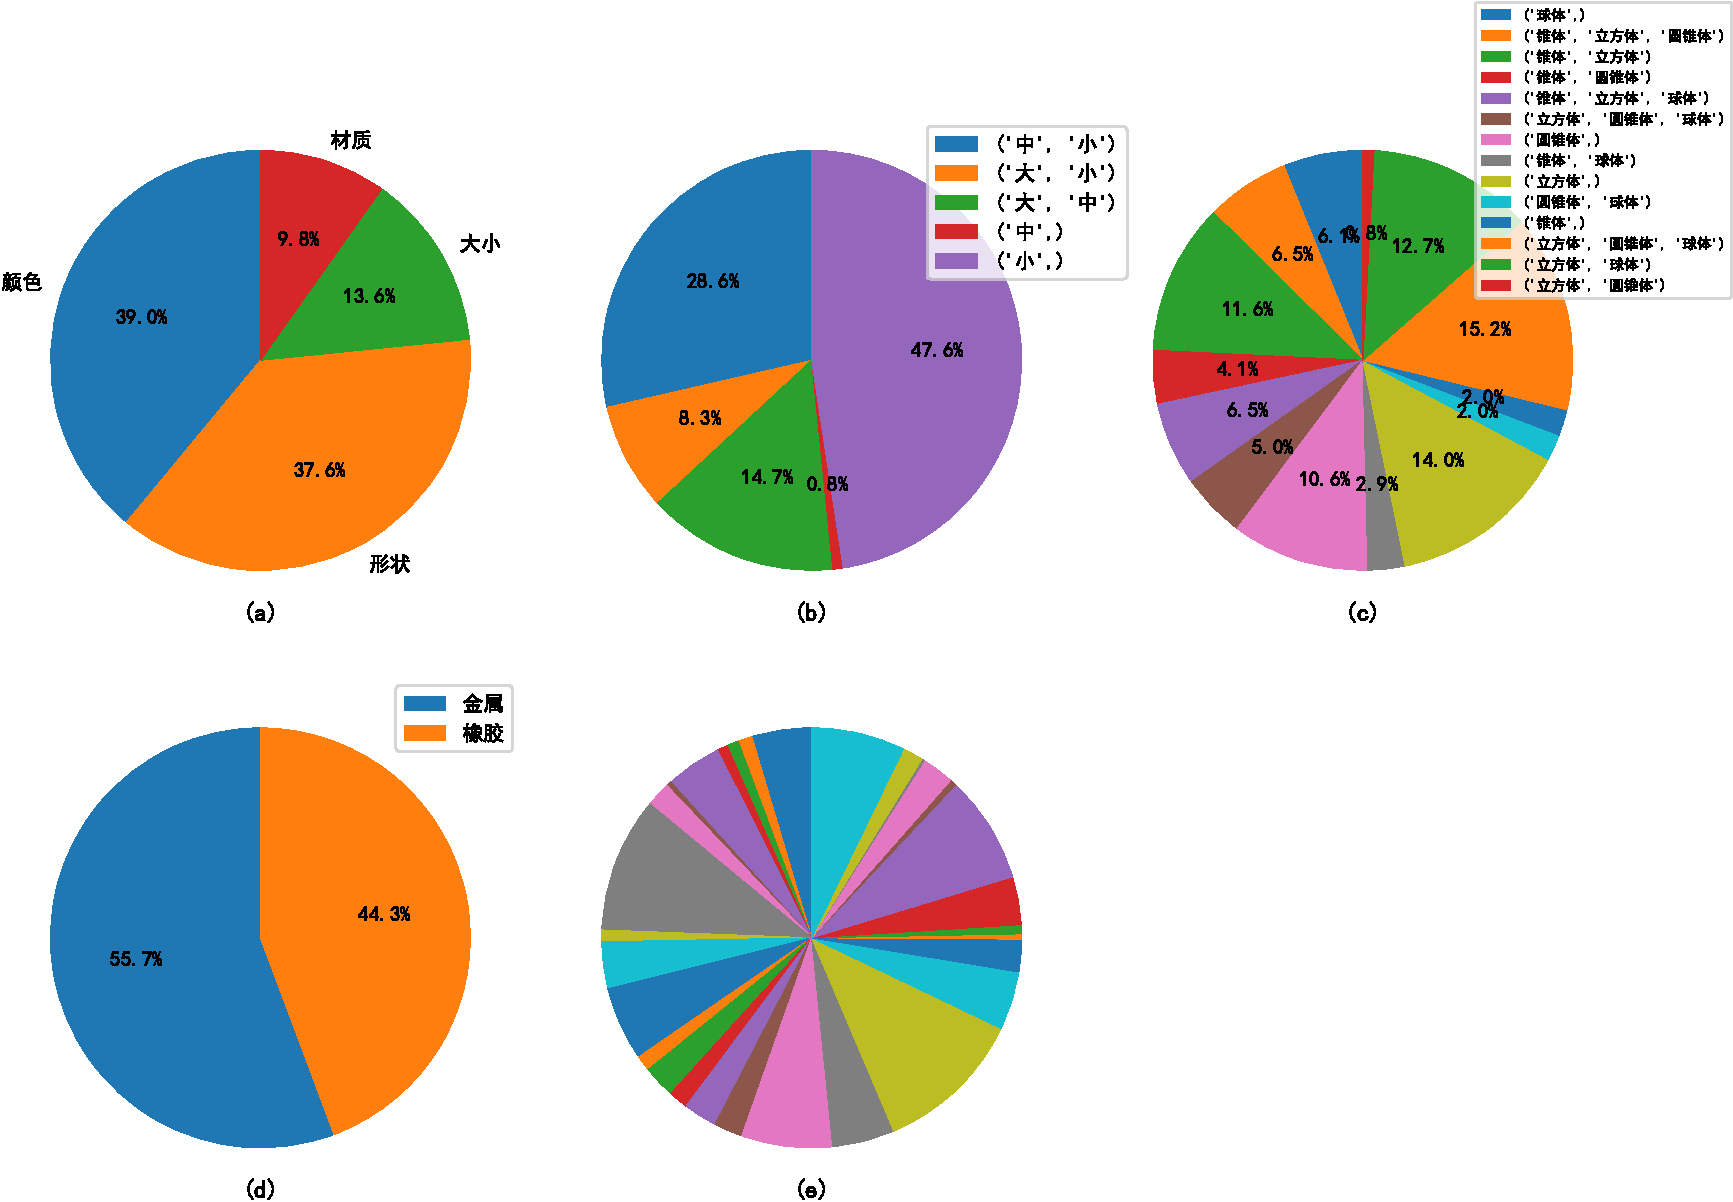
\includegraphics[scale=0.45]{figures/question_distribution-crop.pdf}
    \caption{问题分布统计}
    \label{fig:question_statistics}
\end{figure}

图\ref{fig:template_statistics}(a)中展示了POVQAD中问题在不同问题模板上的分布情况,\ref{fig:template_statistics}(b)中展示
了特定类型问题根据场景中物体数量划分的分布情况。
\begin{figure}[h]
    \centering
    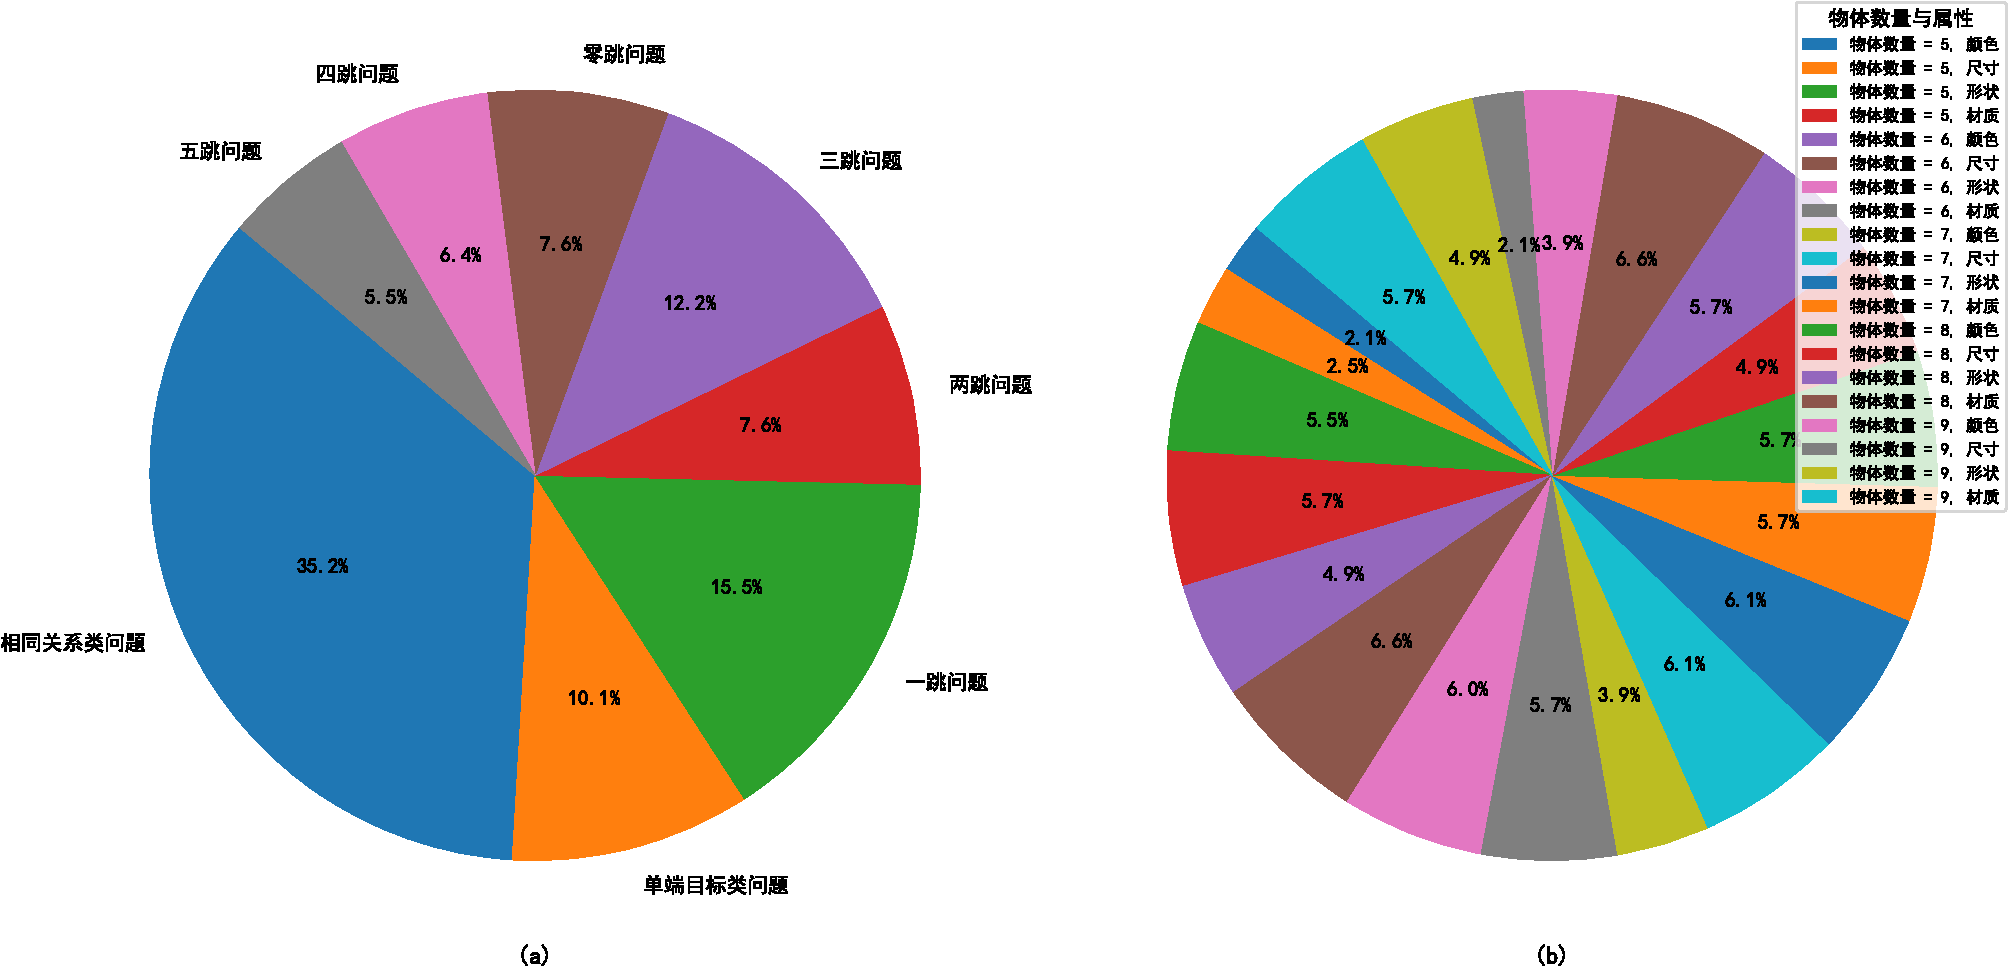
\includegraphics[scale=0.45]{figures/question_template_distribution-crop.pdf}
    \caption{问题模板分布情况}
    \label{fig:template_statistics}
\end{figure}
\subsection{对比实验}
为了证明POVQAD数据集对不同推理能力方法的区分性与挑战性,
本文选取了五种代表性方法在该数据集上进行实验:传统感知模型(CNN+LSTM)、
主流多模态大模型(DeepSeek、Gemini 2.5 Flash、ChatGPT-4o),以及人类作答作为理论上限参考。
每种方法的输入为POVQAD的图像、自然语言问题以及环境约束。实验重复进行三次取平均值,最终实验结果如图\ref{fig:dataset-comparison}所示,可得出如下结论:
\begin{enumerate}[nosep]
\item 数据集具有良好的难度区分能力。各方法在POVQAD上的准确率差异明显,充分体现了模型间的空间理解与逻辑推理能力差距。尤其是传统模型(CNN+LSTM)仅达到 45.4\% 的准确率,明显低于VLMs方法,显示POVQAD对浅层感知模型构成了挑战。
\item 多模态大模型在不完全信息推理方面存在性能瓶颈。
即便是先进的多模态大模型(如 ChatGPT-4o)也未能达到人类水平,
在复杂场景、信息遮挡和规则约束下的准确率仍有明显提升空间,说明POVQAD能有效考察模型对隐含信息与环境规则的建模能力。
\item POVQAD能作为更强推理任务的评估基准。
结果表明,POVQAD能有效区分浅层感知模型与具备显式推理机制的方法,
同时能检测当前主流多模态模型在空间推理与知识补全方面的能力边界,具备良好的基准测试价值。
\end{enumerate}
\begin{figure}[h]
\centering
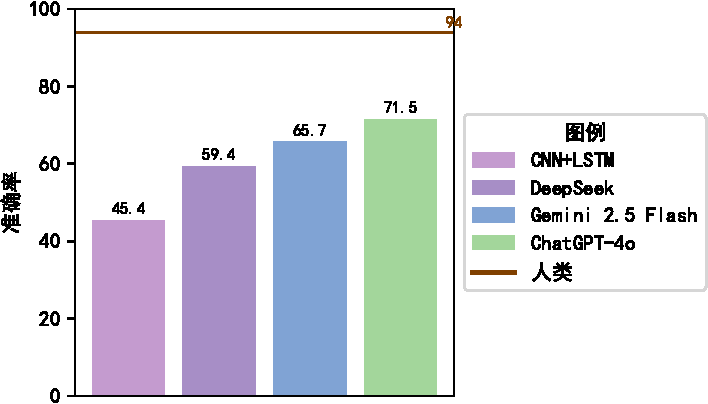
\includegraphics[scale=0.8]{figures/dataset-experiment-crop.pdf}
\caption{不同方法在POVQAD上回答问题的准确率}
\label{fig:dataset-comparison}
\end{figure}
\section{本章小结}
本章聚焦CLEVR数据集的场景完全可见、不要求模型使用外部背景知识进行推理等方面的缺陷,构建一个新的数据集POVQAD,以满足
本文对部分可见积木世界场景下空间推理问答的研究需要。

本章为后续神经符号VQA框架在部分可见积木世界场景下的空间推理问答的实验与分析奠定了坚实的数据基础。